\documentclass[10pt]{article}
\usepackage{graphicx,geometry,amssymb,amsmath,amsfonts}
\usepackage{float}
\restylefloat{table}
\usepackage{lscape}
\usepackage{verbatim,latexsym}
\usepackage{Sweave}
\usepackage{epstopdf}
\usepackage{subfigure}
\usepackage{amsthm,graphicx,wasysym}
%\usepackage{titlesec}
\usepackage[utf8]{inputenc}
\usepackage[english]{babel}
\usepackage{longtable}

\usepackage{color}   % May be necessary if you want to color links and for color text
\usepackage[dvipsnames]{xcolor}



\usepackage{hyperref}
\hypersetup{
    colorlinks=true, %set true if you want colored links
    linktoc=all,     %set to all if you want both sections and subsections linked
    linkcolor=blue,  %choose some color if you want links to stand out
}


\setlength{\parindent}{0em}
\setlength{\parskip}{0em}
\renewcommand{\baselinestretch}{1.0}

\geometry{left=1.25in, right=1.25in, top=1in, bottom=1in}

\title{Comparing $C^r$ Values with Network Perturbation Results; Pintials - No Harvest}
\date{}       
\author{Joanna Bieri, Christine Sample, Brady Mattsson, Darius Semmens, and ...}

\begin{document}
\Sconcordance{concordance:PintailAnalysisReview_6_6_18_NoHarvest.tex:../CodePintails_NewEqn/PerturbationResults_NoHarvest/PintailAnalysisReview_6_6_18_NoHarvest.rnw:%
1 50 1 1 13 42 1 1 4 6 0 1 2 1 1 1 39 31 1 1 18 16 1 1 53 29 1 1 63 29 1 1 52 28 1 1 53 29 1}


\newcommand{\multilineR}[1]{\begin{tabular}[b]{@{}r@{}}#1\end{tabular}}
\newcommand{\multilineL}[1]{\begin{tabular}[b]{@{}l@{}}#1\end{tabular}}
\newcommand{\multilineC}[1]{\begin{tabular}[b]{@{}c@{}}#1\end{tabular}}

\thispagestyle{empty}

\maketitle

\tableofcontents


\section{Pintail Notes and Generalized \texorpdfstring{$C^r$}{CR} }
We model a population of northern pintail waterfowl building our model based entirely on the paper {\it{A modeling framework for integrated harvest and habitat management of North American waterfowl: Case-study of northern pintail metapopulation dynamics}} by Mattsson et. al.

We track the population at three breeding nodes: $AK$, $PR$, and $NU$ and two wintering nodes: $CA$ and $GC$. The population is modeled through three times steps each season:
\begin{itemize}
\item Breeding and Fall Migration: We begin with survival and breeding at $AK$, $PR$, and $NU$, followed by migration toward $CA$ and $GC$. If hunting is included in the model it happens during the fall migration. The breeding rate is density dependent.
\item Winter and Spring Migration/Stopover: Next the migrants survive the winter and migrate toward $PR$ and $AK$. Post harvest survival is density dependent.
\item Final Spring Migration: Some migrants will choose to use $PR$ as a stop over and complete their migration by continuing on to $AK$ or $NU$ from $PR$. The transition probabilities are density dependent and depend on the number of ponds at $PR$.
\end{itemize}

We use a generalized network model formulation were we define one time step as

\begin{equation}
\vec{\mathbf{N}}_{t+1}={\mathbf{A}_t}\vec{\mathbf{N}}_t
\end{equation}

Where $\vec{\mathbf{N}}_{t}$ contains the population at each of the $n$ nodes and $c$ classes at time $t$. The matrix $\mathbf{A}_t$ contains all of the demographic node update and migration data for time $t$. (Christine and Joanna have a draft of a paper with this construction).\\


Within the pintail code we calculate the $C^r$ values for both the origin and the intermediate nodes during each season. We use a generalized one equation definition of $C^r$ in matrix form. {\it{This generalized version is from Joanna and Christine and has not yet been published, currently in draft form. It allows for complete generality in the number of nodes, classes, and seasons.}}

\begin{equation}
\vec{\mathbf{C}}_t=\left(\prod_{\tau=t}^{t+s-1}\mathbf{A}_\tau^T\right)\vec{\mathbf{1}}_{nc}
\end{equation}

where $s$ is the total number of seasons in one anual cycle, for the pintails $s=3$ and $\vec{\mathbf{C}}_t$ is a column vector that contains the $C^r$ values at each node for each class for focal season, or time, $t$. 

We note that because the code is run to equillibrium, the overall growth rate of the nework is equal to one. We can calculate the growth rate using:

\begin{equation}
\lambda_t= \frac{\vec{\mathbf{N}}_t^T}{N_t^{tot}}\vec{\mathbf{C}}_t
\label{lambda}
\end{equation}\\
where $N_t^{tot}$ is the sum of the equilibrium population values across all nodes and all classes in the network and is represented by the following summation
\begin{equation}
N_t^{tot}=\sum_{r=1}^n\sum_{x=1}^{c}N^x_{r,t}
\end{equation}

\section{Baseline Simulation}
% 
The baseline simulation gives us identical results to {\it{A modeling framework for integrated harvest and habitat management of North American waterfowl: Case-study of northern pintail metapopulation dynamics}} by Mattsson et. al. For the case of no harvesting we find that the long term carrying capacity for each node during each season, including all classes, is

\begin{Schunk}
\begin{Soutput}
season 1 : k= 2505506 1797057 1681391 0 0
season 2 : k= 0 0 0 4621049 2260102
season 3 : k= 2318685 3665270 0 0 0
\end{Soutput}
\end{Schunk}



\begin{figure}[H]
\begin{center}
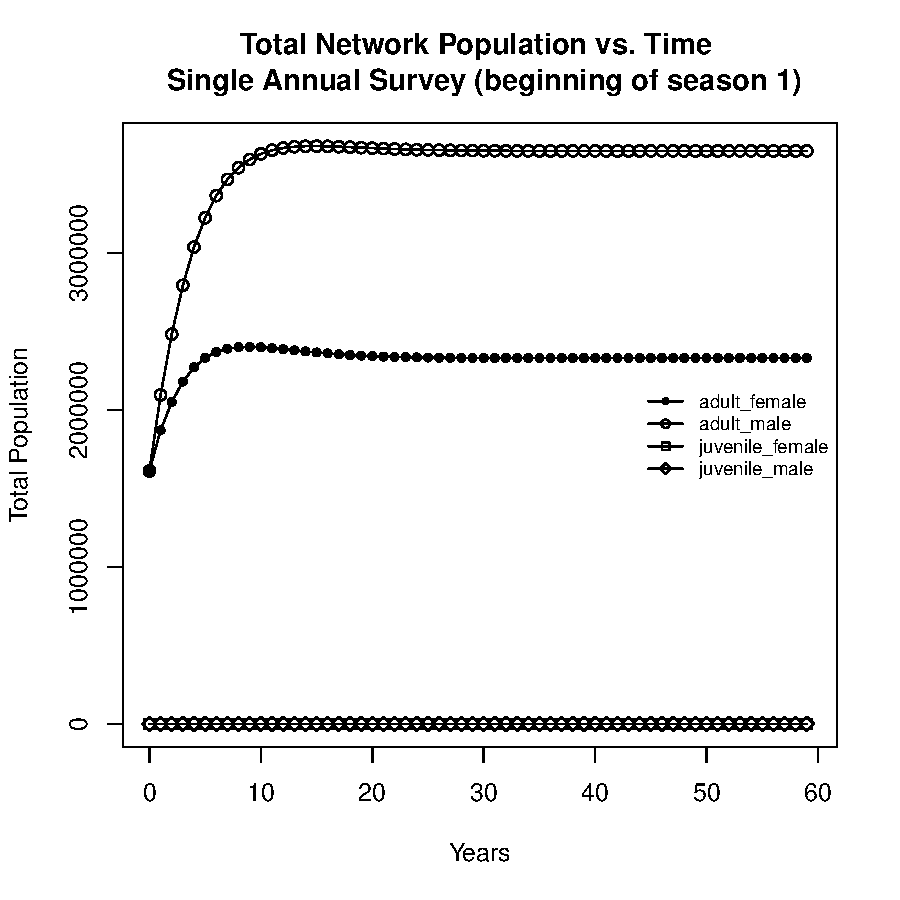
\includegraphics[width=.7\textwidth, height=.6\textwidth]{RGraphics-pintailbaseline}
\caption{Baseline results: population over time at wintering node before breeding.}\label{fig:pintailbaseline}
\end{center}
\end{figure}

\clearpage

%%%%%%%%%%%%%%%%%%%%%%%%%%%%%%%%%%%%%%%%%%%%%%%%%%%%%%%%%%%%%%%%%%%
%%%%%%%%%%%%%%%%%%%%%%%%%%%%%%%%%%%%%%%%%%%%%%%%%%%%%%%%%%%%%%%%%%%
%%%%%%%%%%%%%%%%%%%%%%%%%%%%%%%%%%%%%%%%%%%%%%%%%%%%%%%%%%%%%%%%%%%

\section{Perturbation Experiment - Perturbing Node Survival Rates}

To investigate the utility of the metrics as an indicator of the change in carrying capacity $K$ we consider the following perturbations to the survival rate at each node:

\[PERT = .9, .8, .7, .6, .5\]

Some notes about the simulations:
\begin{itemize}
\item All simulations are run to equillibrium with an error tollerance of within 1 animal, meaning the network growth rate $\lambda=1$.
\item The simulations are run using three seasons (Breading, Winter, and Stopover) to account for densitiy dependent migration in the spring.
\item We preturb survival rates only during Breeding and Winter seasons, since the stop over is not a true season but rather a flyover and in the initial code survival was 100\% during this season.
\end{itemize}
%  


\newpage 




\section{Perturbation Experiment - Perturbing Node Survival Rates}

For the following plots we only perturb Breeding and Winter seasons, keeping survival rates during the flyover at 1. For all $C^r$ values, we still use only Breeding season CR values for AK, PR, and NU and Winter seasons CR values for CA and GC, ignoring the flyover season. 

We will consider new metrics for the x-axis of our graph:
\begin{itemize}
\item Baseline $C^r$ vs $K$ perturbations - this is the population weighted $C^r$ value averaged across classes and averaged across seasons: Figure \ref{fig:pintail_barcr_averageCR}
\item Baseline $W^r$ vs $K$ perturbations - the population proportions during averaged (not weighted) across seasons: Figure \ref{fig:pintail_barcr_WR}
\item Baseline $D_s$ vs $K$ perturbations - the proportional dependence as defined in Bagstad et al, generalizing to account for juveniles: Figure \ref{fig:pintail_barcr_DS}
\item NEW - Baseline Criticality $KR_i$ vs $K$ perturbations - defined as the network growth rate in the absence of node $i$ population weighted average across seasons: Figure \ref{fig:pintail_barcr_KR}. Note that because we are at equilibrium the baseline network growth rate is $\lambda = 1$.
\end{itemize}


\newpage
\subsection{Population weighted average \texorpdfstring{$C^r$}{CR}}

\vspace{-.5cm}
\begin{figure}[H]
\begin{center}
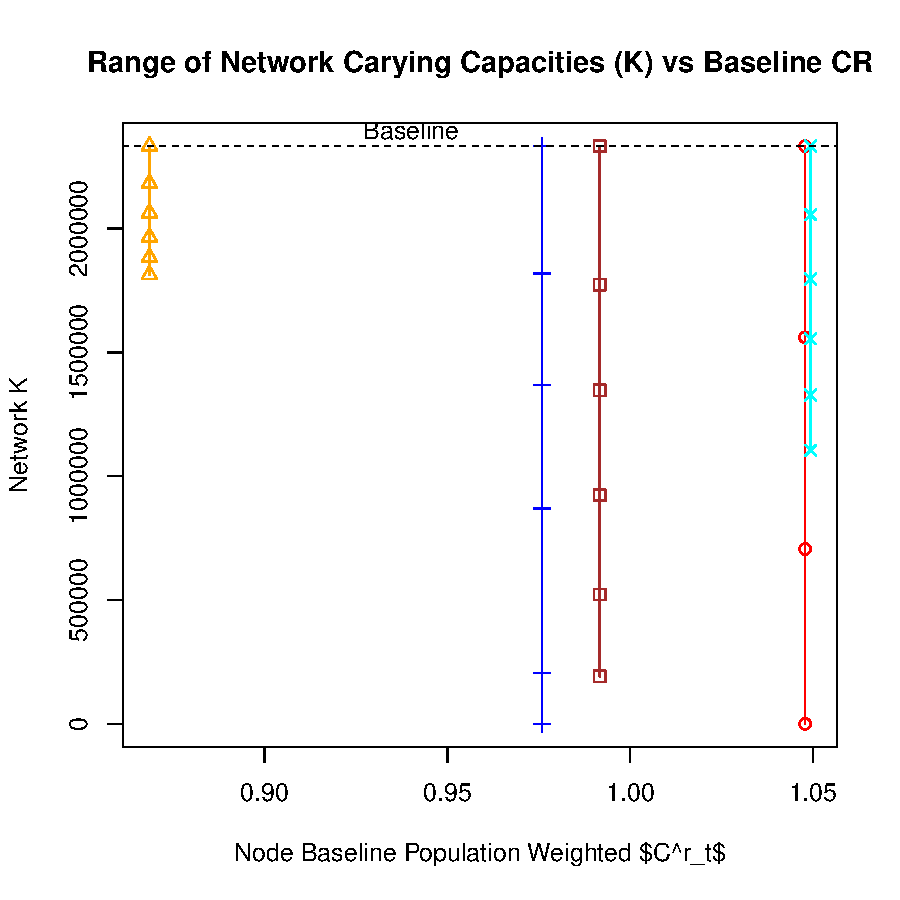
\includegraphics[width=.8\textwidth, height=.8\textwidth]{RGraphics-pintail_barcr_averageCR}
\caption{Perturbation results: Range of K values after perturbations to each node, X-axis represents baseline population weighted $C^r_t$ value for each node}\label{fig:pintail_barcr_averageCR}
\end{center}
\end{figure}

\vspace{-.5cm}
\begin{tabular}{|c|c|c|}
\hline
{\color{Sepia}AK} & $\Box$ & breeding \\
\hline
{\color{red}PR} & $\bigcirc$ & breeding \\
\hline
{\color{orange}NU} & $\triangle$ & breeding \\
\hline
{\color{blue}CA} & $+$ & winter \\
\hline
{\color{cyan}GC} & $\times$ & winter \\
\hline
\end{tabular}

\vspace{1cm}
The $C^r$ values are calculated using a population weighted average for the classes within the nodes and the generalize matrix form of $C^r$. Each node has adult females, adult mapes, juvenile females, and juvenile males.

\newpage
\subsection{Population Distribution \texorpdfstring{$W^r$}{WR}}


\vspace{-.5cm}
\begin{figure}[H]
\begin{center}
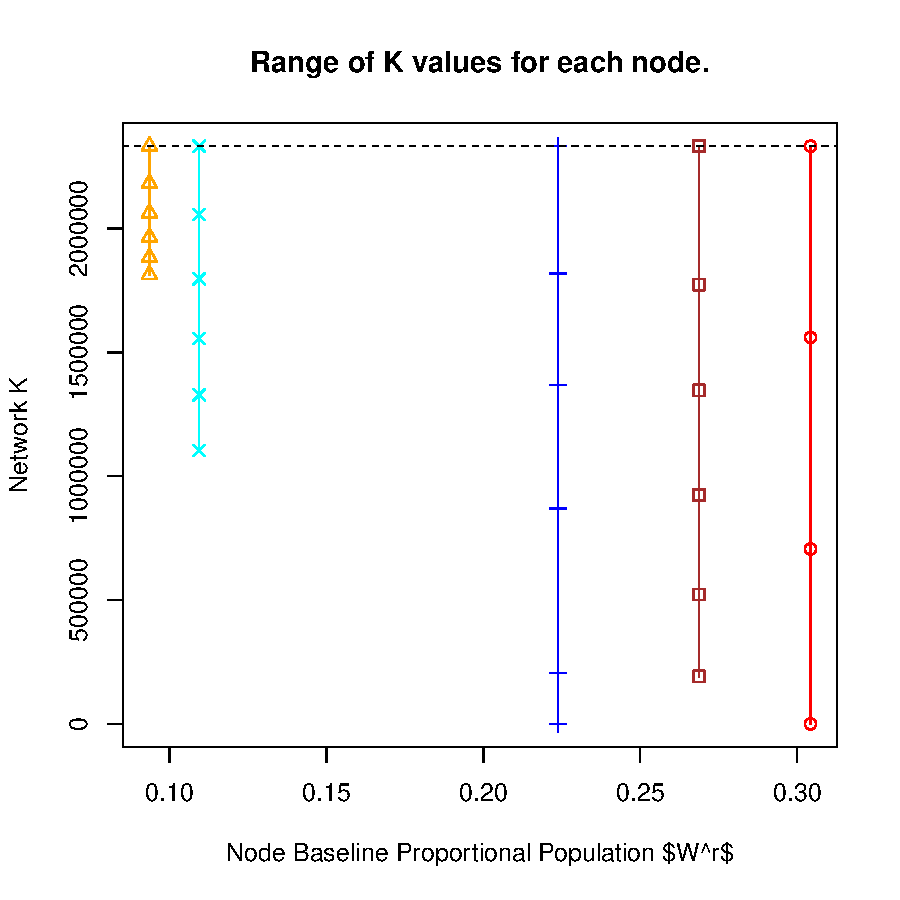
\includegraphics[width=.8\textwidth, height=.8\textwidth]{RGraphics-pintail_barcr_WR}
\caption{Perturbation results: Range of K values after perturbations to each node, X-axis represents baseline $W^r$ value for each node}\label{fig:pintail_barcr_WR}
\end{center}
\end{figure}

\vspace{-.5cm}
\begin{tabular}{|c|c|c|}
\hline
{\color{Sepia}AK} & $\Box$ & breeding \\
\hline
{\color{red}PR} & $\bigcirc$ & breeding \\
\hline
{\color{orange}NU} & $\triangle$ & breeding \\
\hline
{\color{blue}CA} & $+$ & winter \\
\hline
{\color{cyan}GC} & $\times$ & winter \\
\hline
\end{tabular}

\vspace{1cm}
$W^r$ is calculated as the percent of the total population residing at a node. From the breeding season we get values for AK, PR, and NU and from the winter season we get values for CA and GC.

\newpage
\subsection{Proportional Dependence \texorpdfstring{$D_s$}{DS}}


\vspace{-.5cm}
\begin{figure}[H]
\begin{center}
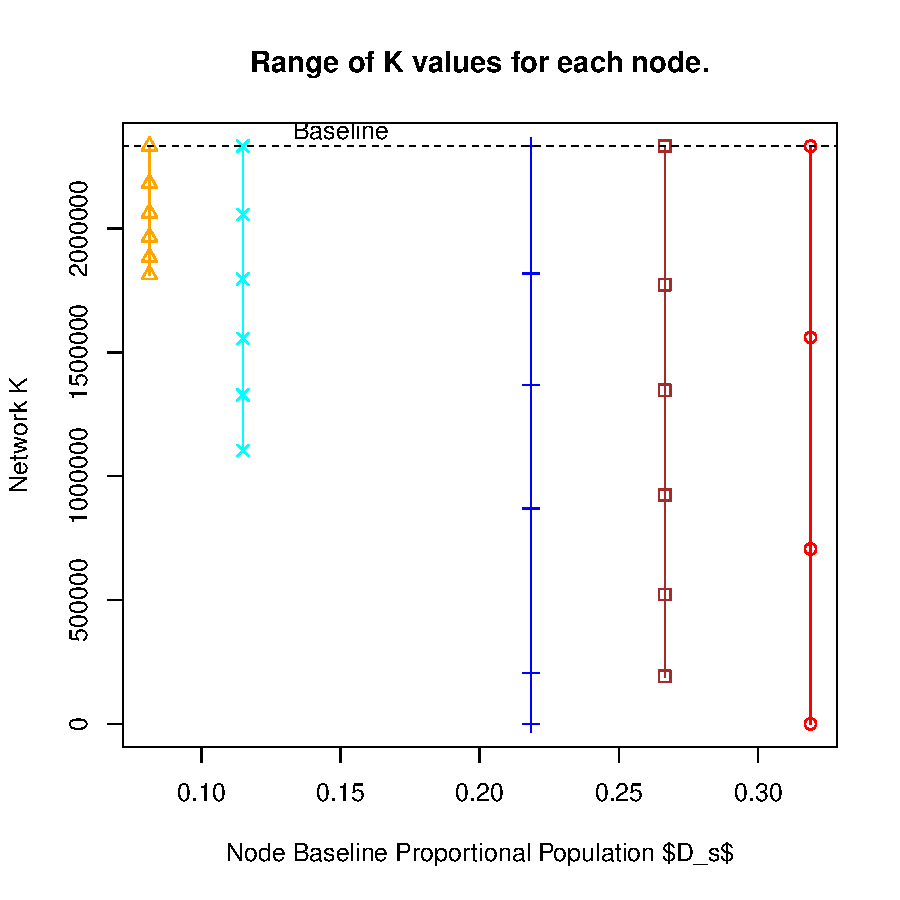
\includegraphics[width=.8\textwidth, height=.8\textwidth]{RGraphics-pintail_barcr_DS}
\caption{Perturbation results: Range of K values after perturbations to each node, X-axis represents baseline $D_s$ value for each node}\label{fig:pintail_barcr_DS}
\end{center}
\end{figure}

\vspace{-.5cm}
\begin{tabular}{|c|c|c|}
\hline
{\color{Sepia}AK} & $\Box$ & breeding \\
\hline
{\color{red}PR} & $\bigcirc$ & breeding \\
\hline
{\color{orange}NU} & $\triangle$ & breeding \\
\hline
{\color{blue}CA} & $+$ & winter \\
\hline
{\color{cyan}GC} & $\times$ & winter \\
\hline
\end{tabular}

\vspace{1cm}
$D_s$ is calculated following Bagstad et al. We first find the population weighted $C^r$ values for each of the seasons and then average across the anual cycle.

\newpage
\subsection{Criticality - NEW \texorpdfstring{$K^r$}{KR}}

\vspace{-.5cm}
\begin{figure}[H]
\begin{center}
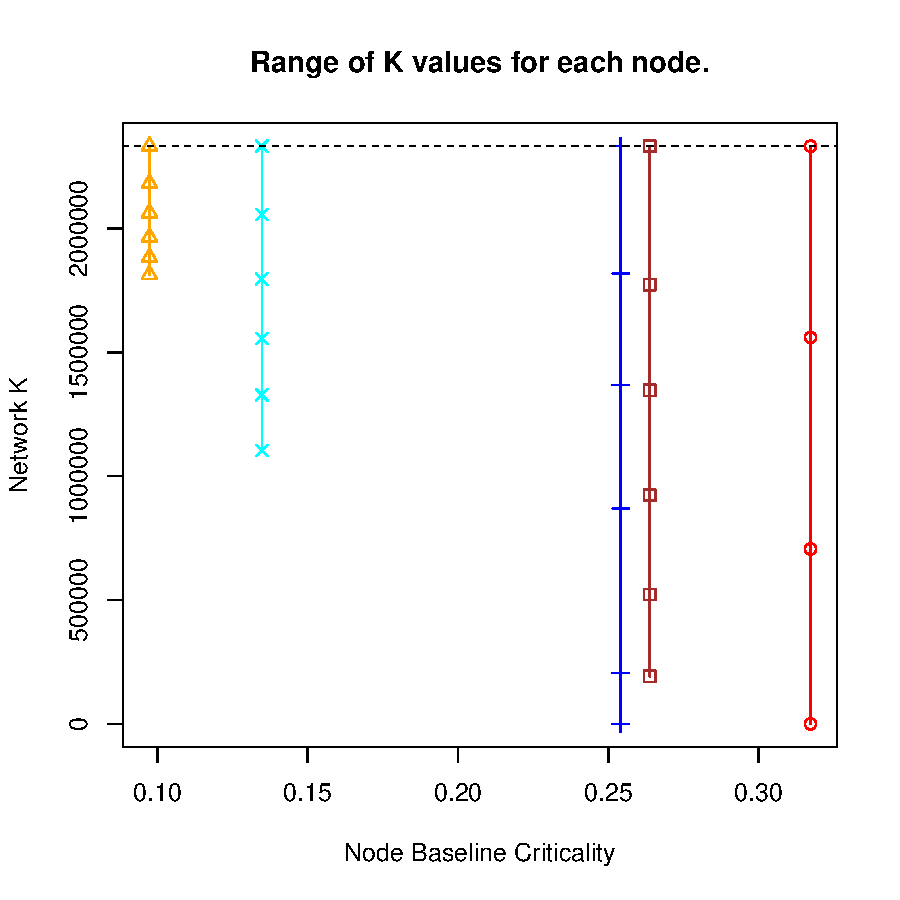
\includegraphics[width=.8\textwidth, height=.8\textwidth]{RGraphics-pintail_barcr_KR}
\caption{Perturbation results: Range of K values after perturbations to each node, X-axis represents baseline Criticality value for each node}\label{fig:pintail_barcr_KR}
\end{center}
\end{figure}

\vspace{-.5cm}
\begin{tabular}{|c|c|c|}
\hline
{\color{Sepia}AK} & $\Box$ & breeding \\
\hline
{\color{red}PR} & $\bigcirc$ & breeding \\
\hline
{\color{orange}NU} & $\triangle$ & breeding \\
\hline
{\color{blue}CA} & $+$ & winter \\
\hline
{\color{cyan}GC} & $\times$ & winter \\
\hline
\end{tabular}

\vspace{1cm}
Criticality $K^r$ is a new metric concieved of by Christine and her colleagues. The basic idea is that from $C^r$ we can calculate the network growth rate $\lambda$. In the case of a population in equilibrium, like our simulations, $\lambda = 1$. Then one could also calculate a theoretical $C^r$ value as if on of the nodes was removed. From this theoretical $C^r$ value we could calulcate a new network growth rate $\gamma$. We define criticality as 
\[K^r = \lambda - \gamma \]
In other words $K^r$ represents the amount of the network growth rate that flows through the focal node $r$. In our equilibrium case is $K^r=1$ then all of the network growth rate must flow through $r$ and removal of $r$ reduces the new growth rate $\gamma$ to zero. Alternatively, if $K^r=0$ then none of the original network growth rate flows through $r$ and removal of $r$ does not change the growth rate, $\lambda=\gamma=1$.

\end{document}
